\chapter{Digital Communication Methods} \labchap{digital_communications}
Now that we have converted the analog sensor reading into the digital realm, we have to move the data around to use it.
There are many communication methods that utilize a variety of protocols, but for simplicity we will be discussing three of the most common in small digital circuits.
Each of these methods utilize ``Transistor-Transistor-Logic'' or TTL voltages, meaning the signals use 0V for a logical 0, and any other voltage above a threshold is considered a logical 1.
Each method is also known as a serial communication method as each bit in the message is communicated in series.

\section[UART Explained]{Universal Asynchronous Receive and Transmit} \labsec{uart}
The Universal Asynchronous Receive and Transmit (UART) bus is a full-duplex digital communication method where the receiver and transmitter of information can transmit asynchronously. 
This is one of the simplest communication interfaces as a controller only needs to pull the data bus to the ``low'' state at certain intervals while transmitting.
There is no addressing or synchronization required, so the transmitter can just ``shout'' the bits down the line and does not care if the receiver gets them or not.
Since its asynchronous, both the receiver and transmitter must agree on the baudrate, or bits-per-second, beforehand and will set their own internal clocks to the appropriate speed.
By timing the arrival of ``low'' or ``high'' signals, the controllers can interpret data in the transmission packet.
If the baudrates are not synchronized properly, the interval between the bits will be different and data will become corrupted at either end.
Further reading can be done at Analog Dialogue \cite{AnalogDialogue:UART}.

\begin{figure}[h!]
    \caption[UART protocol diagram]{The UART protocol diagram with a small waveform example. 
    Courtesy of Eric Pena and Mary Grace Legaspi \cite{AnalogDialogue:UART}.}
    \labfig{uart_protocol}
    \centering
    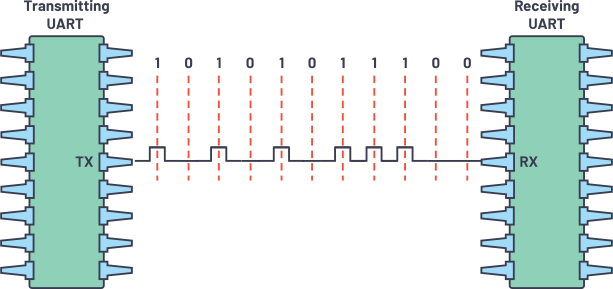
\includegraphics[height=2.5in]{appendices/digital_communication/uart_protocol.png}
\end{figure}

\section[I2C Explained]{Inter-Integrated Circuit} \labsec{i2c}
The I2C, or Inter-Integrated Circuit, communication bus is most commonly used for slower speed transmissions between integrated circuits on a circuit board.
It is a synchronous, multi-nodal, half-duplex topology which means that multiple controllers and responders can exist on the same bus and communicate, but not simultaneously.
I2C uses two pins for communication, one for data (SDA) and one for clock (SCK).
Unlike UART, I2C devices do not need to agree on a clock speed before communication begins, the clock line speed is adjusted by the controller and all devices automatically synchronize to it.
Additionally, I2C devices have a one-byte address that distinguish them and allow for a controller to request data from a specific responder.
This limits the number of unique devices on an I2C bus to 255 and can create some problems if multiple I2C devices of the same address are present.
For the latter problem, I2C multiplexing solutions exist to mitigate the issue \footnote[3]{https://www.adafruit.com/product/2717}.

To begin a message, the controller will initialize a start condition on the line then broadcast the desired device address.
This lets all devices on the bus know that the controller wants to talk with a specific device.
The controller will then follow-up with a one-byte data frame.
Depending on the responder's programming, it will respond with another data frame that the controller will receive.
a typical example of this is a controller querying a device for the value of a register in its memory.
Further reading can be done at Analog Devices \cite{AnalogDevices:I2C}.

\begin{figure}[h!]
    \caption[I2C protocol diagram]{The I2C protocol diagram with a successful write byte transmission. 
    Courtesy of Sal Afzal \cite{AnalogDevices:I2C}.}
    \labfig{i2c_protocol}
    \centering
    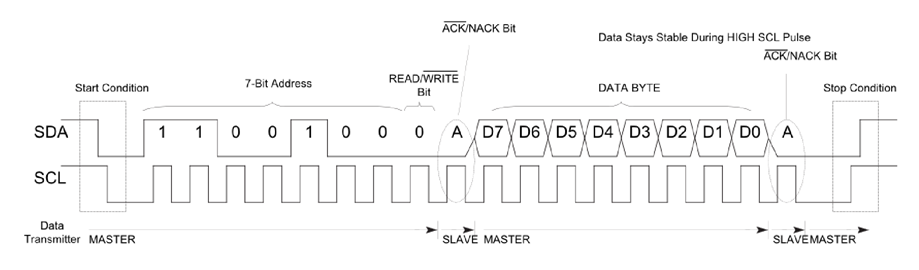
\includegraphics[width=\textwidth]{appendices/digital_communication/i2c_protocol.png}
\end{figure}

\section[SPI Explained]{Serial Peripheral Interface} \labsec{spi}
The Serial Peripheral Bus (SPI) is the slightly modified version of the UART protocol.
SPI introduces clock synchronization so that a main and subnode do not have to agree on a communication rate beforehand and also allows multiple subnodes to be present on the same bus.
By toggling an enable pin, the main node can tell a subnode to ignore or respond to a request on the data line.
SPI uses four lines to communicate: Main Out Sub In (MOSI), Main In, Sub Out (MISO), Clock (SCK), and Chip Select (CS).
A typical multi-subnode topology is shown in the figure below.

To begin a message, the main node will pull the CS pin for the desired subnode low and send out a message on the MOSI line.
When the subnode receives the message, it can respond depending on its programming.
In the case of a data storage unit like RAM or an SD card, the subnode will just write data to a specified register from the main node's message.
If the subnode is a sensor, it may respond with the value from one or more registers in its memory.
More reading can be done at Analog Dialogue \cite{AnalogDialogue:SPI}.

\begin{figure}[h!]
    \caption[SPI protocol diagram]{The SPI protocol diagram with a successful write byte correspondence. 
    Courtesy of Piyu Dhaker \cite{AnalogDialogue:SPI}.}
    \labfig{spi_protocol}
    \centering
    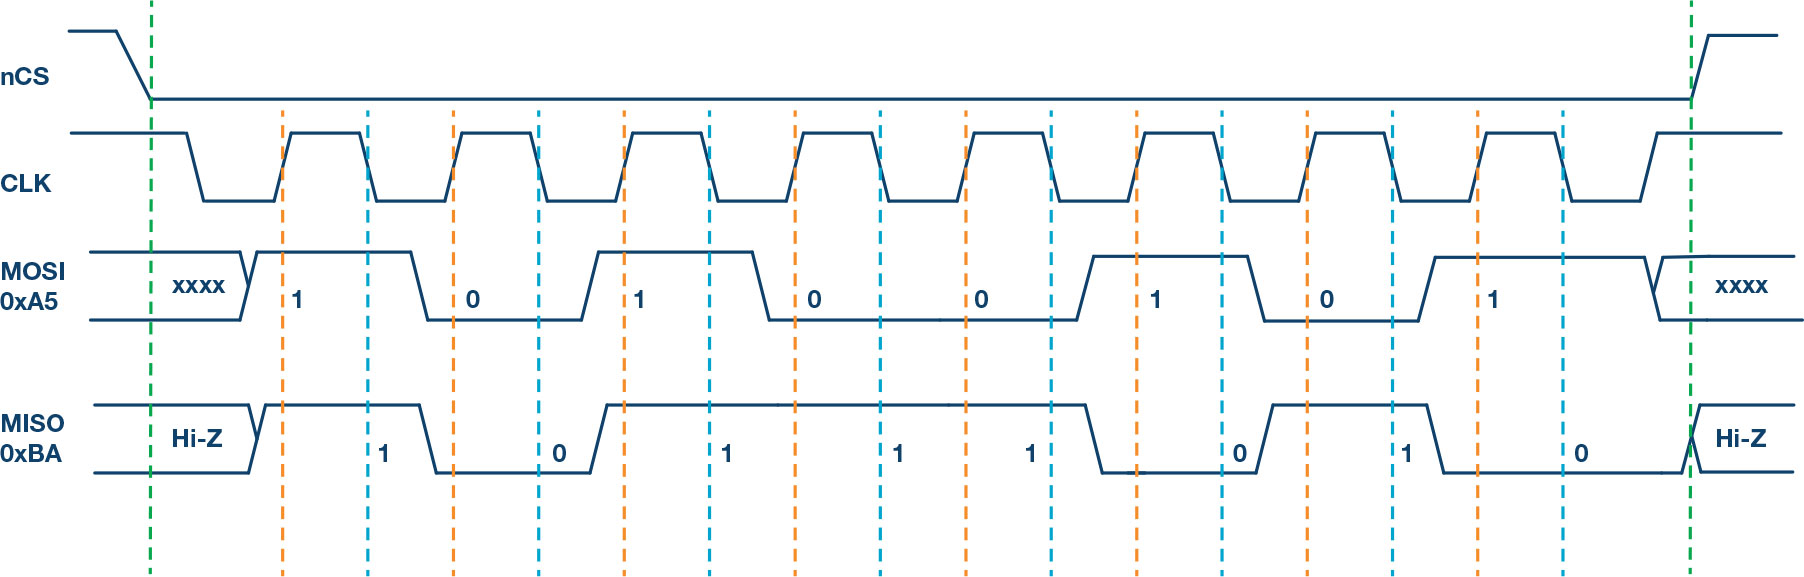
\includegraphics[width=\textwidth]{appendices/digital_communication/spi_protocol.jpg}
\end{figure}
